\documentclass[11pt]{beamer}
\title{Array Fold Logic Proof} 
\usepackage{verbatim}
\usepackage{amsmath}
\usepackage{amsthm}
\usepackage{listings}
\usepackage{graphics}
\usepackage{color}
\usepackage{stmaryrd}\usefonttheme[onlymath]{serif}

\newtheorem{proposition}{Proposition}
\date{\today}


\begin{document}
\maketitle
\begin{frame}\frametitle{Overview }
\begin{itemize}
\item  Overview of the proof.


\item Proof of Complexity.


           
\end{itemize}
\end{frame}
\begin{frame}\frametitle{Definitions}
\begin{definition}[SMC]
A symolic $k$-counter machine is a tuple $\mathcal{M} = (\mathbf{\eta}, X, Q, \delta, q^{init})$, where 
$\delta \subseteq Q \times \textsc{CC}_k(X) \times \texttt{IC}(X) \times Q \times \mathbb{Z}^k$.

\end{definition}
\begin{definition}[Translation]
We define a translation of a functional constant $f$ of $\texttt{FSort}^m$ as an SCM $\mathcal{M}(f) = (\mathbf{\eta}, X, Q, \delta, q^{init})$. Let $G = \langle S, E, \gamma\rangle$ be the edge-labeled graph of $f$, then the translation... 
\end{definition}

\end{frame}

\begin{frame}\frametitle{Definitions}
\begin{center}
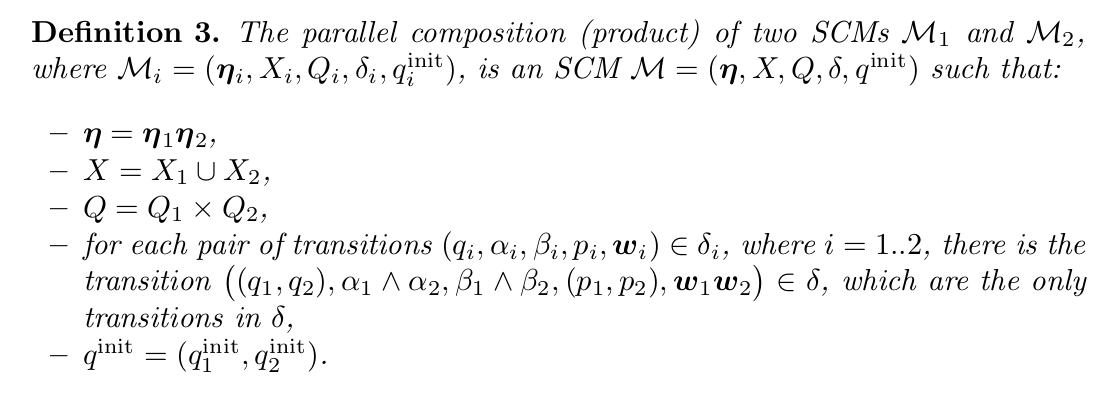
\includegraphics[scale=0.28]{para.png}
\end{center}
\end{frame}


\begin{frame}\frametitle{Small Model Property}
\begin{lemma}
There exists a constant $c\in \mathbb{N}$, such that an AFL formula $\Phi$ is satisfiable iff there exists a model $\sigma$ it maps each variable in $X$ to integer that $\le 2^{|\Phi|^c}$ and array to sequence of $\le 2^{|\phi|^c}$ where each integer of the array also lies in the bound.
\end{lemma}


\end{frame}

\begin{frame}\frametitle{Complexity}


\begin{theorem}
The satisfiability problem of AFL is \textbf{PSPACE}-complete.

\end{theorem}
\begin{itemize}
\item Membership:
If the small model property holds, an NTM can
\begin{itemize}
\item nondeterministically guess variable use space of $|\Phi|^c$ bits.
\item guess one-by-one the value of $2^{|\Phi|^c}$ array cells and use $|\Phi|^c$ bits to count the current index.
\item due to the bound of the variable and the bound of length, the counter value of fold is also bounded in poly.
\end{itemize} 

Then a NTM can simulate the SAT problem in \textbf{PSPACE}.








\item Hardness:
Reduce the emptiness problem of intersection of DFAs which is \textbf{PSPACE}-complete to this problem.

\[\bigcap_{i = 1}^n \mathcal{L}(A_i)\ne \emptyset\]


$A_i$ can be simulated by $fold^i_a$ with a single counter: What is the alphabet? What is accepting? Why this work?
\end{itemize}

\end{frame}



\begin{frame}\frametitle{Proof of Small Model Property}

Given a array $a$ and a assignment $\sigma$, assume $\sigma$ satisfiy $\phi$.

Let $s = |\psi| \le 3|\phi|$.


\[\mathcal{R} = \{[0, c_1], [c_1,c_1], [c_1 + 1, c_2 - 1], [c_2, c_2], \ldots, [c_l, +\infty]\}\]

Size of $\mathcal{R}$: $2dim(\mathbf{c}) + 1 \le 3s$.


A \textit{mode}: is a tuple in $\mathcal{R}^k$ that describes the region of each counter.

Reversal-bounded: $\mathcal{M}$ is reversal-bounded, then any run can traverse at most $max = r\cdot k \cdot |\mathcal{R}| \le \mathcal{O}(s^3)$ different modes.

Take an accepting run $Tr = Tr_1\cdots Tr_{max} $ of $\mathcal{M}$.

The property of $Tr_i = \delta_m, \cdots, \delta_n$. How to modify $Tr_i$ to get $\bar{Tr_i}, Tr_i^*$.




\end{frame}


\begin{frame}\frametitle{Proof of Small Model Property}

The satisfiability of $\phi$ then can be translated into a LP problem $\mathbf{LP} = \bigwedge_{i = 1}^{5}\mathbf{LP}_i$, where

$\mathbf{LP}_1$: 
\begin{center}
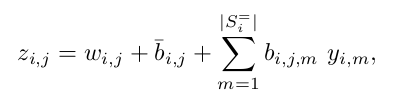
\includegraphics[scale=0.4]{lp1_1.png}

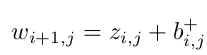
\includegraphics[scale=0.4]{lp1_2.png}
\end{center}


$\mathbf{LP}_2$: not fold(copy of variables).

$\mathbf{LP}_3$: link fold and not fold. 

$\mathbf{LP}_4$: bound of counters.


$\mathbf{LP}_5$: all input constraint in $Tr$ are satisfiable.

Then we get an LP problem, which by [1] the model is bounded.

[1]C. H. Papadimitriou. On the complexity of integer programming. 

\end{frame}


\iffalse
\begin{frame}\frametitle{Pushdown Automata}
\begin{definition}[PDA]
A pushdown automaton is a tuple $M = (Q, \Sigma, \Gamma, \delta, q_0, Z, F)$.
\begin{itemize}
\item $\delta$ is a finite subset of $Q\times (\Sigma \cup \{\epsilon\}) \times \Gamma \times Q \times \Gamma^*$.
\item $\Sigma, \Gamma$ are the tape alphabet and stack alphabet respectively.
\item $Z$ is the initial symbol of stack representing the bottom of the stack.
\end{itemize}

\end{definition}

\end{frame}
\begin{frame}\frametitle{One-Counter Automata and Pushdown Automata}

\textbf{One-counter automata is a special case of pushdown automata.}

$\Gamma = \{Z, g\}$ and the stack of PDA can be written as 

\[Zg^n, n\in \mathbb{N}\]

which can be regarded as a non-negative counter.



\end{frame}


\begin{frame}\frametitle{Two-Counter Automata is Turing Equivalent}
Proof sketch:
\begin{enumerate}
\item A Turing machine can be simulated by two stacks.
\item A stac kcan be simulated by two counters. Where one counter is used to storing the binary number represented by the stack and the other one used for scratchpad for update. 

\item Four counters can be simulated by two counters. Four virtual counter $a,b,c,d$ can be encoded as a G\"odel number $2^a3^b5^c7^d$ by one real counter and the comparablyother counter is used as scratchpad.
\end{enumerate}
\end{frame}

\begin{frame}\frametitle{Undecidable problem of TM}
\begin{itemize}
\item Acceptance problem. $\langle TM, \omega\rangle$.
\item Reachability problem. $TM, c_{init}, c_{f}$.

\end{itemize}
More generally, Rice's theorem formally state what problem is decidable about turing machine.

\begin{theorem}{Rice's Theorem}
If $P$ is a non-trivial property, and the language holding the property, $L_P$ is recognized by a turing machine $M$, then $L_P = \{\langle M\rangle\mid L(M) \in P\}$ is undecidable.
\end{theorem}


Hence, some important basic problems are all undecidable for counter automata.
\end{frame}


\begin{frame}\frametitle{Several Ways to Retain the Decidability}
\begin{itemize}
\item Restrict to 1-counter automata.

\item Structural restriction: flatness (no nested cycles).

\item Reversal Boundness.
\end{itemize}
\end{frame}


\begin{frame}\frametitle{Reachability Problem of OCA}

\begin{definition}[Configuration of OCA]
Given an OCA $\mathcal{A} = (Q, q_0, F, \Delta, \epsilon)$, we use a pair $(q, c)$ represent the configuration of $\mathcal{A}$.

\end{definition}

The semantic of an OCA can be regarded as a labelled transition system where the states are the configurations of $\mathcal{A}$ and the transitions are induced from $\Delta$ and $\epsilon$.


\textbf{REACHABILITY PROBLEM:}

Given an oca $\mathcal{A}$ and two configurations $(s, c_s), (t, c_t)$, whether we can find a feasible run of transition system $T_{\mathcal{A}}$ such that $(s,c_s)\rightarrow_{\mathcal{A}}^*(t,c_t)$.


\end{frame}


\begin{frame}\frametitle{Complexity of OCAReach Problem}

\begin{theorem}[Haase's Phd]
Reachability problem in one-counter automata is NP-complete.
\end{theorem}

\end{frame}

\begin{frame}\frametitle{Algorithm}
Why the reachability of OCA is hard?

\end{frame}

\begin{frame}\frametitle{Idea of the algorithm}
\begin{itemize}
\item Path and path flow.
\item Weight and drop of a path.
\item Support.
\item Edge decomposition.
\item Type-1, Type-2 and Type-3 certificate.
\end{itemize}

\end{frame}
\fi
\end{document}